% !TeX root = ../main.tex
\graphicspath{{Figures/Results}}

\chapter{Results}\label{ch:results}

\section{Classification Performance}\label{results:sec:model_perf}
Following training and post-hoc threshold tuning, model performance was evaluated across 15 anti-TB drugs using sensitivity, specificity and F1 score. Four weight schemes were compared: TB-Profiler (baseline for our model), WHO catalogue (baseline for our weights), WHO updated with expert rules (WHO+ER), and the updated catalogue augmented with filtered variants from FN samples (WHO+ER+Filtered). For each weight scheme, hollow circles denote naiive performance prior to any training or threshold tuning, with only binary weights extracted from the catalogues. Their color-filled circles represent performance post-training and threshold application (Figures~\ref{fig:sens,fig:spec, fig:f1}).

\subsection*{Sensitivity}
Across all 3 weight schemes, sensitivity matched or exceeded TB-Profiler for 13 out of 15 drugs (Figure~\ref{fig:sens}). The untrained baseline anchors highlight sensitivity gains occur post-training and threshold application, rather than catalogue makeup alone, all filled markers sit above their hollow anchors. Under the WHO catalogue baseline, sensitivity increased for all 15 drugs, post-training and threshold tuning. WHO+ER improved for 13 out of 15 drugs, and WHO+ER+Filtered improved for 14 out of 15 drugs. Across most drugs, comparing the three weight schemes, performance was broadly similar. However, there were notable exceptions such as moxifloxacin, where WHO+ER achieved the highest sensitivity among weight schemes. Another drug is delamanid, where both WHO+ER and WHO+ER+Filtered outperformed WHO baseline, suggesting that that catalogue updates with expert rules and FN harvested variants provided meaningful contributions. For bedaquiline, catalogue via expert rules and filtered variants produced the most substantial sensitivity boost out of all drugs, consistent with its newer status in anti-TB treatment.

Clofazimine, delamanid, and linezolid posed a significant challenge to the model, with all weight schemes hitting a ceiling of 0.65 post-training and threshold application. Nevertheless, all WHO weight schemes showed improved performance over TB-Profiler profiler, suggesting the probabilistic framework being able to extract signals even with a smaller set of resistant cases. 

\begin{figure}[H]
  \centering
  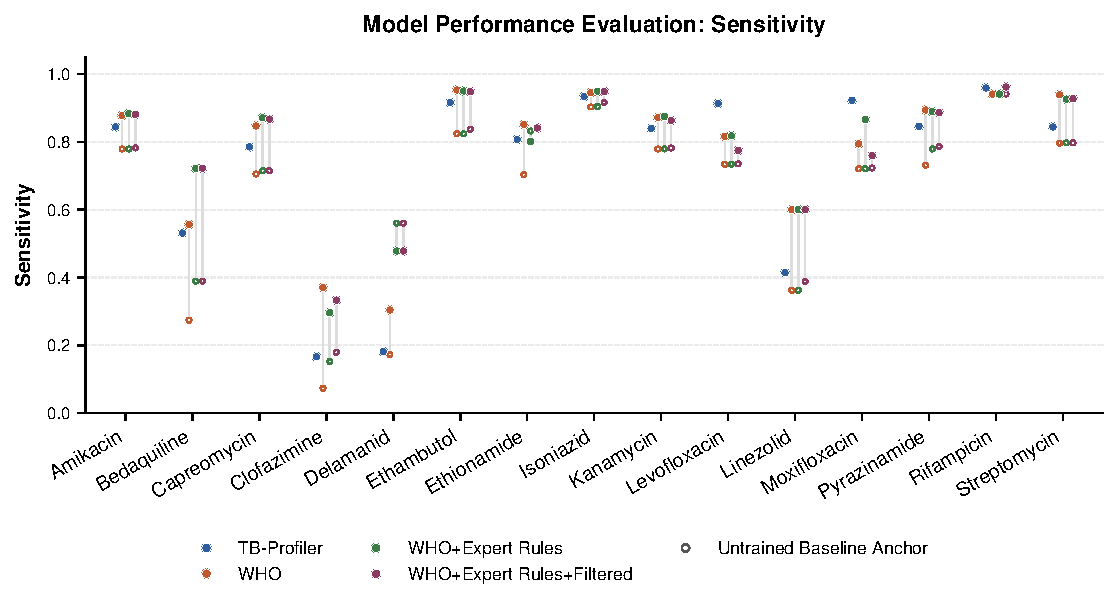
\includegraphics[width=\textwidth]{figures/sensitivity.pdf}
  \caption{Sensitivity of the neural network with tb-profiler as the baseline, WHO, and WHO augmented with
  expert rules, and filtered is shown aswell. The naive pass with only the catalogues encoded as 1s , or 0s
  is shown as empty circles, and the trained model results are filled in.}\label{fig:sens}
\end{figure}

\subsection*{Sensitivity}

As stated in Section 2.5, the threshold tuning procedure enacted a hard specificity boundary of 0.8, and this is visible in Figure~\ref{fig:spec}.
For 8 out of 15 drugs, the learned weights schemes approached or slightly penetrated this floor, illustrating the sensitivity-specificity trade-off accounted for during threshold application. Despite this, ethambutol, clofazimine, delamanid, isoniazid, levofloxacin, moxifloxacin, and ethionamide, specificity for the model weight schemes hovered around TB-Profiler's performance. For rifampicin, the weight schemes matched or even slightly exceeded TB-Profiler's specificity. Subsequently, a specificity difference of $-0.2$ between TB-Profiler and the weight schemes can be observed for amikacin, bedaquiline, capreomycin, kanamycin, pyrazinamide, streptomycin, and linezolid. This gap is a direct manifestation of the specificity trade-off made when boosting sensitivity, ultimately reflecting a higher FP rate, with lowered FN.

\begin{figure}[H]
  \begin{center}
    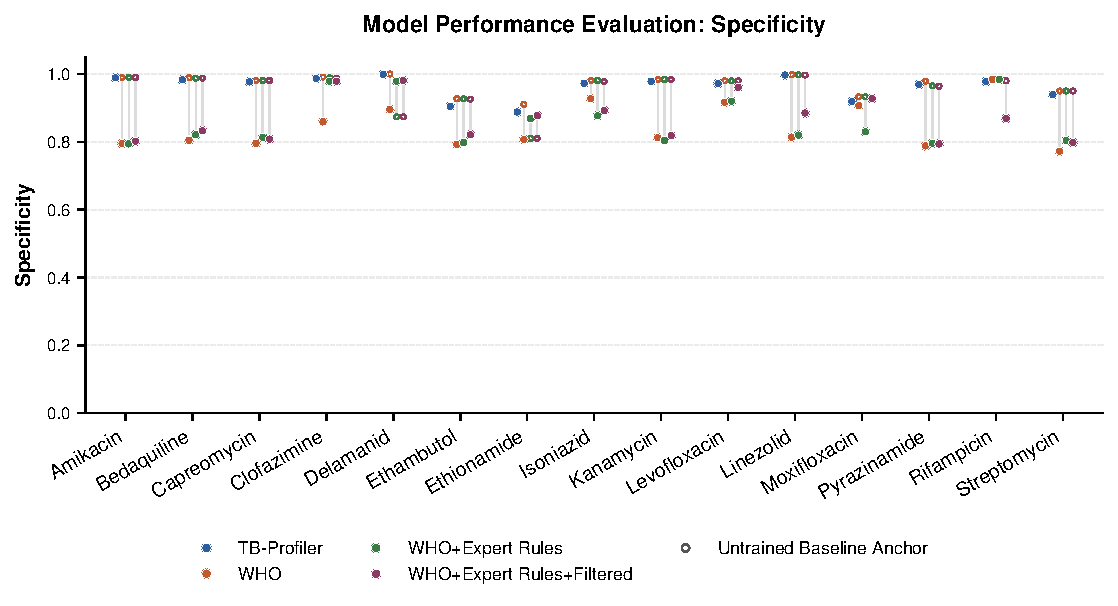
\includegraphics[width=\textwidth]{figures/specificity.pdf}
  \end{center}
  \caption{Specificity of the neural network after training for 15 Anti-TB drugs that had at final confidence
  grading of 1 or 2. TB-profiler (blue) acts as the baseline to show how the neural networks perform with different
  weights. Weights were constructed from the WHO catalogue, and then augmented with expert rules and filtered snps.
  These are represented as hollow circles, and after training, they are represented as filled circles.}\label{fig:spec}
\end{figure}

\subsection*{F1 Score}
The specificity-sensitivity trade-off is reflected in the F1 scores (Figure~\ref{fig:f1}). Drugs where the largest drops in specificity, also showed the largest drops in F1 post-training and threshold tuning: amikacin, bedaquiline, capreomycin, kanamycin, linezolid, and pyrazinamide. This suggests that sensitivity gains were not substantial enough to offset specificity losses under the harmonic mean (F1). The remaining drugs, showed slightly improved or stable F1 compared to TB-Profiler. Clofazimine, delamanid, ethambutol, and rifampicin all showed F1 improvements compared to TB-Profiler. Isoniazid, ethionamide, streptomycin, and moxifloxacin F1 scores remained stable and close to TB-Profiler. Overall, the WHO weight schemes matched or exceeded F1 for 8 out of 15 drugs, demonstrating that specificity costs incurred via threshold tuning does not uniformly degrade overall Classification quality. Lastly, the probabilistic framework provides meaningful gains for drugs where the resistant data is sparse or the WHO catalogue has coverage gaps for. 

\begin{figure}[H]
  \begin{center}
    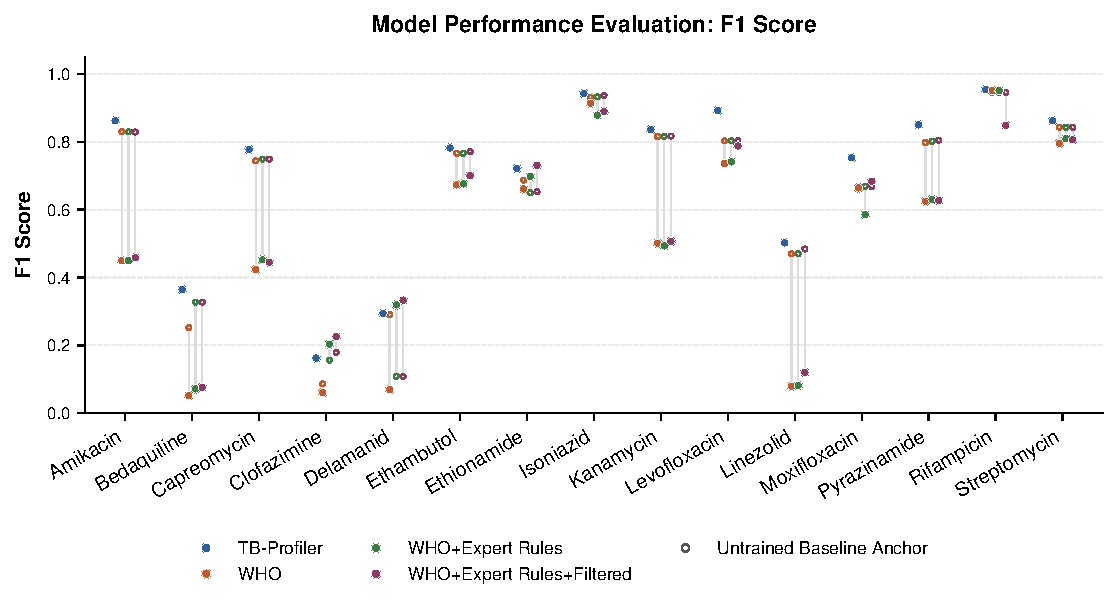
\includegraphics[width=\textwidth]{figures/f1.pdf}
  \end{center}
  \caption{F1 scores of the neural networks, with F1 being the balanced average between specificity and sensitivity.
  In this plot, TB-profiler is used as a baseline, colored in blue, and the untrained networks with shown with hollow
  circles. The trained models are shown with filled circles.}\label{fig:f1}
\end{figure}

\subsection{Training Performance and Convergence}
Training performance was assessed using masked binary cross-entropy loss, AUC, and F1 score over 50 epochs for all weight schemes, here we discuss the WHO+ER+Filtered weight scheme performance (Figure~\ref{fig:filerlr}). Learning curves for other weight schemes and their respective per-drug learning curves can be found in Appendix C. 

Training loss decreased rapidly over the first 20 epochs, falling from approximately 0.500 to near 0.340, before stabilising over the remaining 30 epochs at approximately 0.325. Validation loss followed a close, parallel trajectory, beginning at 0.475, and plateauing around 0.350 with a final test loss of 0.348. Proximity of train, validation, and test loss (within 0.025 of each other) indicates the model generalises well to unseen data without overfitting. Rapid initial descent and stable plateauing over the final 30 epochs are consistent with the expected catalogue weighted scheme performance: the model starts from a biologically grounded position, and requires relatively smaller gradient updates to reach a local minimum. 

Validation AUC climbed from 0.930 at epoch 1 to 0.947 at epoch 50, with training AUC moving from 0.915 to 0.955 over the same interval. Test AUC of 0.9465 falls within training-validation envelope and confirms AUC gains during training reflects effective learning rather than overfitting to training data. Similar to the loss curve, the majority of AUC occurred in the first 20 epochs, following stabilisation. This supports the model reaching its representational capacity early, given the catalogue prior. 

F1 score replicated the same pattern of immediate ascent followed by plateau, with training F1 jumping from $\sim$8.40 to 0.860 and validation F1 from $\sim$0.842 to $\sim$0.857 over 50 epochs, yielding a test F1 of 0.8541. The modest improvement in F1, $\sim$0.060 over 50 epochs, can be understood via the catalogue-weighted models. Catalogue-initialised weights encodes a strong prior, so baseline F1 is expected to be significantly higher than random weights. Training, via gradient-based weight refinement, increments F1 scores which is reflected in the train-validation gap of $\sim$0.003 at convergence. When collated, the loss, AUC, and F1 trajectories indicate an effective training regime with rapid convergence, stable generalisation, and absence of overfitting. The properties are mostly to attribute the biological grounding provided by catalogue weight initialisation and anchor regulariser constraining weight drift during training. 

\begin{figure}[H]
  \begin{center}
    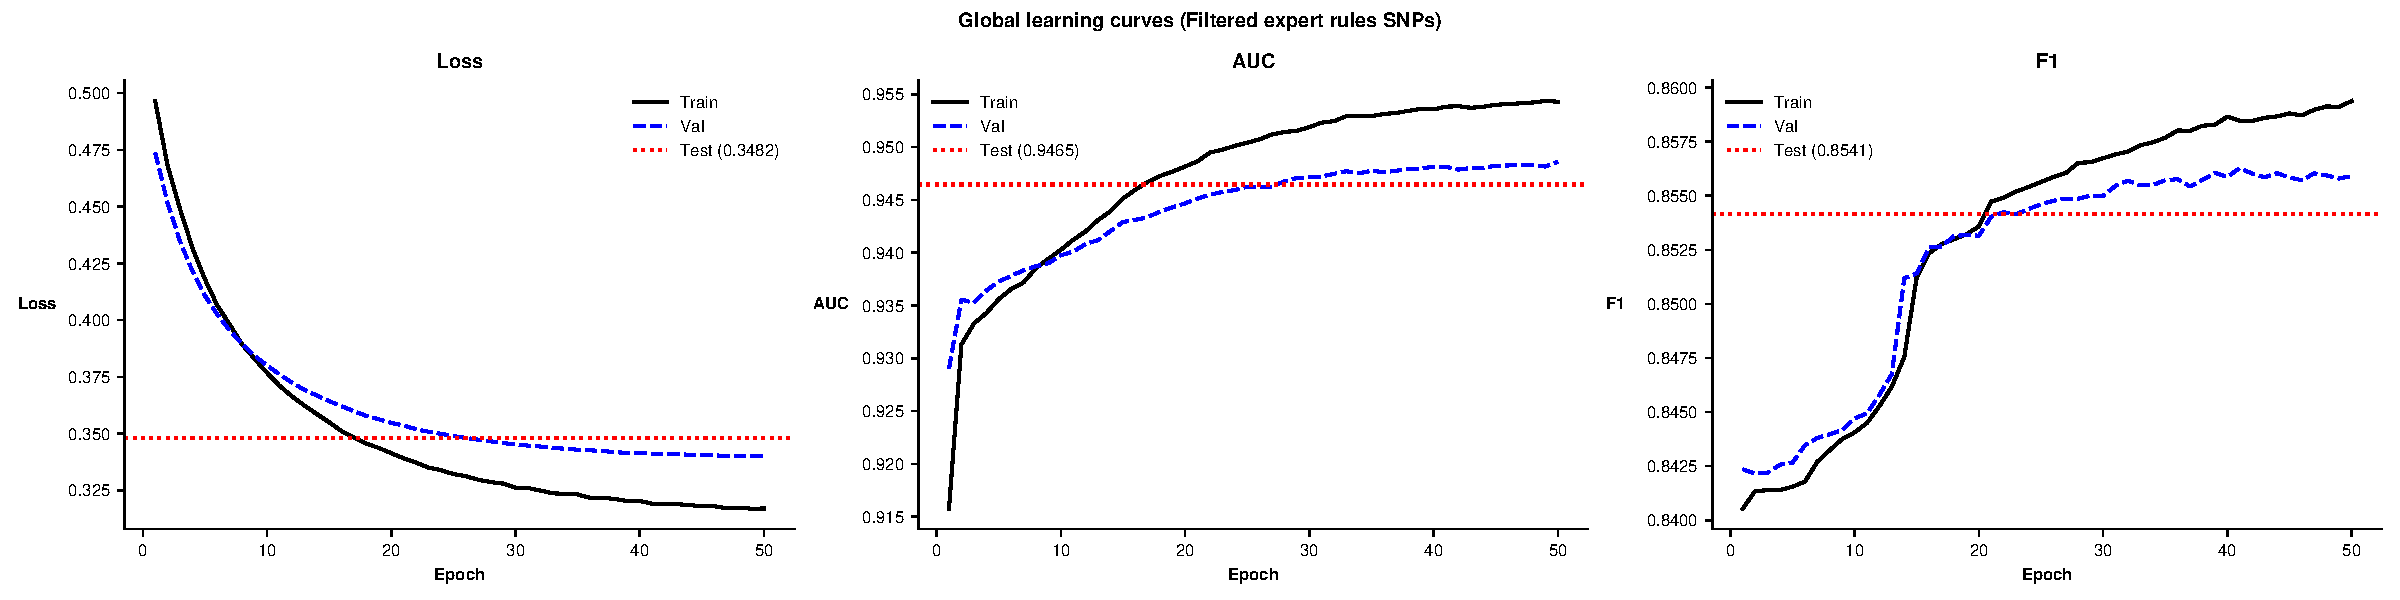
\includegraphics[width=\textwidth]{figures/filtered_expert_rules_learning_curves.pdf}
  \end{center}
  \caption{Global learning curves for er+who catalogue.}\label{fig:filerlr}
\end{figure}

\section{Candidate Mutations}
As per the filtering process outlined in Section [REF], variants from FN samples that were statistically significantly ($-log_{10}(p)>5$) and associated with resistance ($log_{10}(OR)>0$) were selected. Following selection, they were assesed for their inclusion in known lineage markers and in the current ER-updated WHO catalogue scheme. 

Following selection, these variants met two fates: inclusion in what would become WHO+ER+Filtered weight scheme, or for further assessment regarding their candidature as a novel resistance-conferring variant. In this section, for all anti-TB drugs in this dataset, the variants that passed the filtering protocol are displayed in volcano plots in the figures below. The plots are displayed with the $log_{10}(OR)$ in the $x$-axis and the $-log_{10}(p)$ in $y$-axis that were produced during the Fisher's exact test, where the FN samples were `experimental' group and TN the control. The significance and association thresholds are drawn in each plot, creating four quadrants. Top-left houses significant variants not associated with resistance (blue), top-right houses variants that are both associated with resistance and significant (red). Furthermore, the variants the passed the filtering protocols are encircled by a black border (red and black border). Green markers in the graph represent samples with an infinite OR or p-value, due to the variant being present exclusively in resistant or susceptible samples. Variants that produced a sensitivity drop larger than or equal to $5\%$ are annotated, with their gene, polymorphism, and change in sensitivity ($\Delta$Sensitivity). This provides a measurement of the variant's independent predictive contribution, and therefore these variants are of highest priority for validation. The lower left and right quadrants show variants not associated and associated with resistance, but not significant.

Certain volcano plot annotations, and more broadly, filtered variants do not appear to have a name and are deemed the moniker `gene-not-found`. This not suggest an intergenic region, as it has its own annotation, but rather the variant position lacks a human-readable $\texttt{gene=}$ attribute. This tag is common for hypothetical proteins with no assigned gene symbol, \ppe family genes with just a locus tag, and non-coding RNA. This issue can be rectified by locus tag cross-referencing with the TubercuList or PATRIC database [CITE]. They are not discarded as variants in `gene-not-found` locations may be in proximity of genes housing resistance-conferring variants. Resolution of these unknown genes is of high priority for variants that dropped sensitivity steeply post-ablation.

\subsection*{First-line Drugs}

As per Figure~\ref{fig:1st}, the first-line anti-TB agents produced the most-dense plots across all drug classes. Isoniazid, rifampicin, ethambutol and pyrazinamide, displayed many significant variants associated with resistance, highlighted by dense top-right quadrants. Furthermore, on average, the first-line drugs displayed the most outlined variants in the top-right quadrant. 

For isoniazid, the variants that were highlighted from the ablation process were, \textit{katG} C>G, yielding a sensitivity drop of $6.26\%$ when ablated. Furthermore, a `gene not found', a genomic coordinate that is unnamed, had a C>T substitution with a sensitivity drop of $4.56\%$ when ablated. Lastly, an $rpoB$ C>T SNP, in a gene that encodes the drug-target for rifampicin showed an almost borderline decrease in sensitivity of $0.73\%$.

For rifampcin, all annotated variants were located in $rpoB$, the drug-target encoding gene for rifampicin. First of the annotated candidates, $rpoB$ C>T produced a 14.99$\%$ sensitivity drop when ablated. Furthermore, the SNP had approximate $-log_{!0}(p) \approx 120$ and $log_{10}(OR) > 3$, highlighting a 1000-fold enrichment in resistant sample, making it one of the largest sensitivity contributing variants of the first-line drugs. This SNP is followed by $rpoB$ A>T ($\Delta$Sensitivity = 3.37$\%$), $rpoB$ C>G ($\Delta$Sensitivity = 1.22$\%$) and $rpoG$ C>T (different position) ($\Delta$Sensitivity = 1.26$\%$) which is denoted by green box.

Ethambutol yielded the most diverse set of ablated variants of the first line drugs. All annotated variants were in $embB$, drug-target encoding gene for Ethambutol, which is an arabinosyltransferase, essential for arabionogalactan synthesis [CITE]. The filtered variants that met or exceeded the sensitivity-drop threshold were $embB$ A>G (Position= 4247429, $\Delta$Sensitivity= 2.56$\%$, FNP= 95$\%$, RSM= 2$\%$), A>G (Position = 4247847, $\Delta$Sensitivity= 0.66$\%$, FNP= 90$\%$, RSM= 2$\%$), G>C ($\Delta$Sensitivity= 0.97$\%$, FNP= 80$\%$, RSM= 2$\%$), G>A ($\Delta$Sensitivity= 1.05$\%$, FNP=) and A>C ($\Delta$Sensitivity= 1.77$\%$, FNP= 100$\%$, RSM= 2$\%$, green marker) (Figure, Table). Two highly significant SNPs $rpoB$ C>T ($\Delta$Sensitivity= 2.33$\%$) and $katG$ C>G ($\Delta$Sensitivity= 0.97$\%$) were observed. These are likely confounders as the gene products of $rpoB$ or $katG$ are not involved in ethambutol's mechanism of action. Although they are highly significant (p-values $\sim 10^{-140}$) compared to $embB$ variants ($5 \leq$ p-values $\leq 60$), they have relatively modest association with ethambutol resistance (10-fold associated with resistance compared to $embB \geq 10$ with resistance). Additionally, variants in the \ppe gene family were observed with variants in $PE-PGRS$4, 6, 7, 9, and 19 and $PPE$54, 55, and 60 (Table).

To conclude the first-line drugs, pyrazinamide did not produce any ablated variants that passed the sensitivity-loss threshold. However, pyrazinamide produced a large, densely populated plot with many significant variants with positive associations (Figure~\ref{fig:1st}). This can be observed in the filtered variants, where in the pyrazinamide FN samples, the novel variants were in the \ppe family. Variants in $PPE$54, 55 and 60, and $PE-PGRS$4 and 9 can be observed (Table). 

\begin{figure}[H]
    \centering
    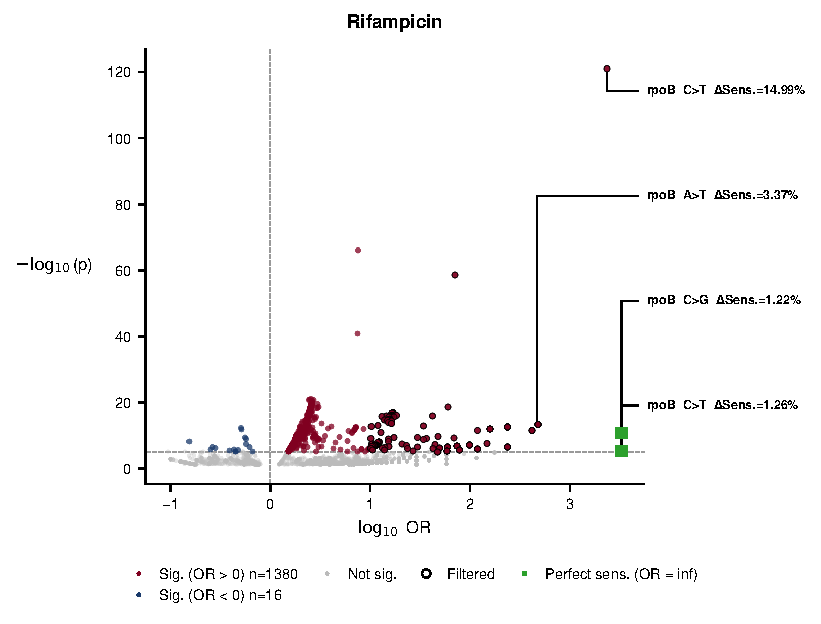
\includegraphics[width=0.45\textwidth]{./figures/plots/rifampicin_volcano.pdf}
    \hfill
    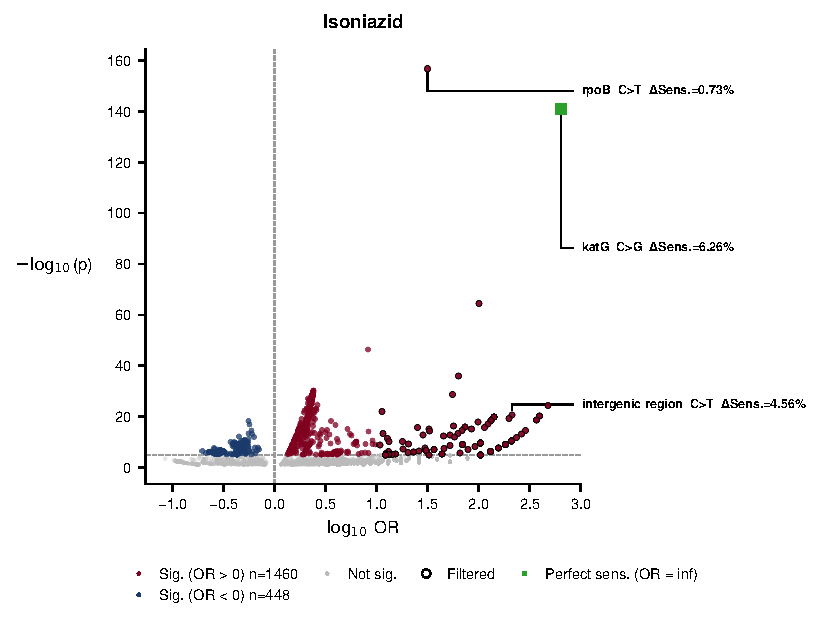
\includegraphics[width=0.45\textwidth]{./figures/plots/isoniazid_volcano.pdf}
    \hfill
    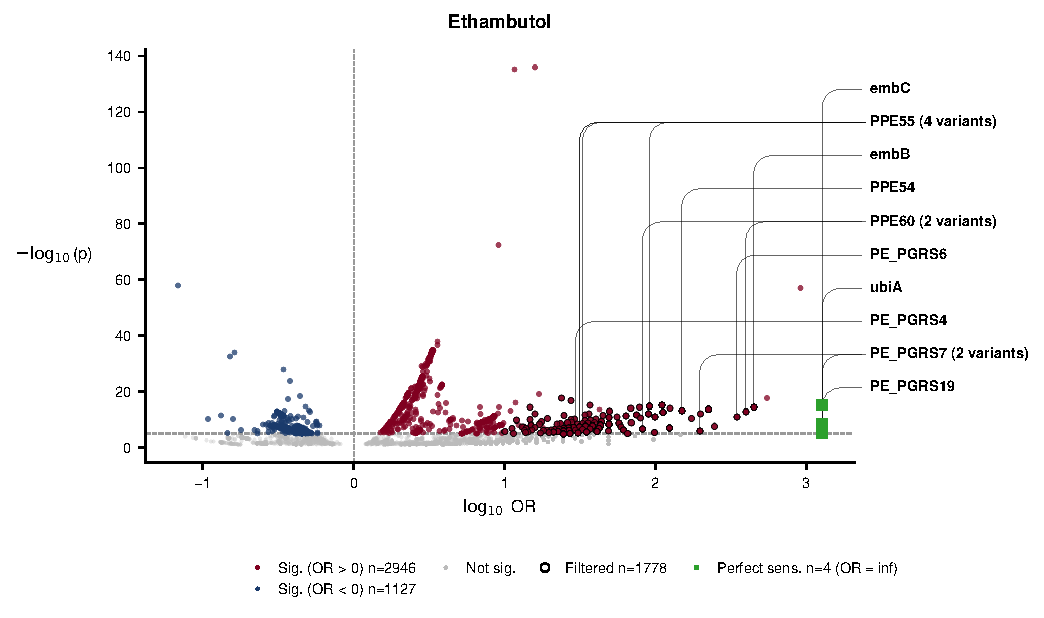
\includegraphics[width=0.45\textwidth]{./figures/plots/ethambutol_volcano.pdf}
    \hfill
    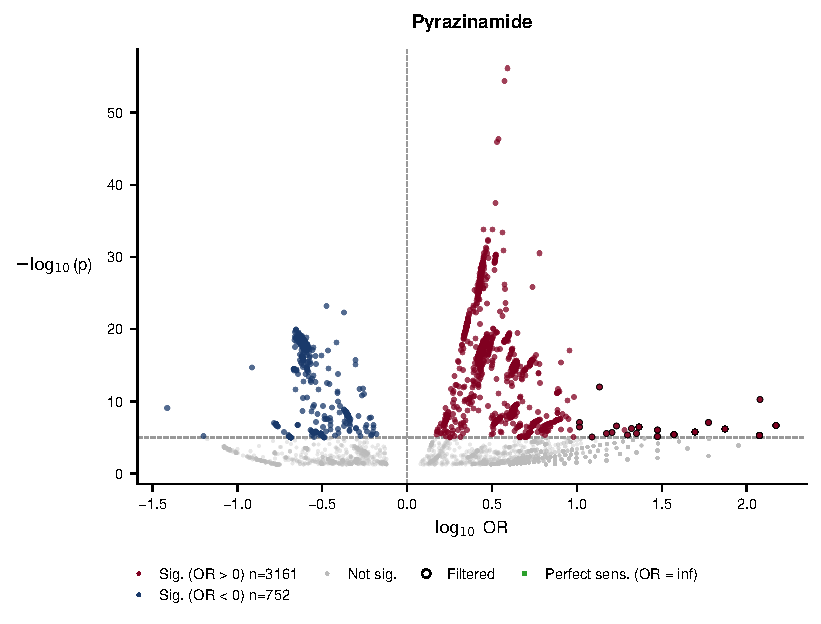
\includegraphics[width=0.45\textwidth]{./figures/plots/pyrazinamide_volcano.pdf}
    \hfill
  \label{fig:1st}
\end{figure}

\subsection{Second-line Drugs}

\subsubsection{Group A}

\begin{figure}[H]
    \centering
    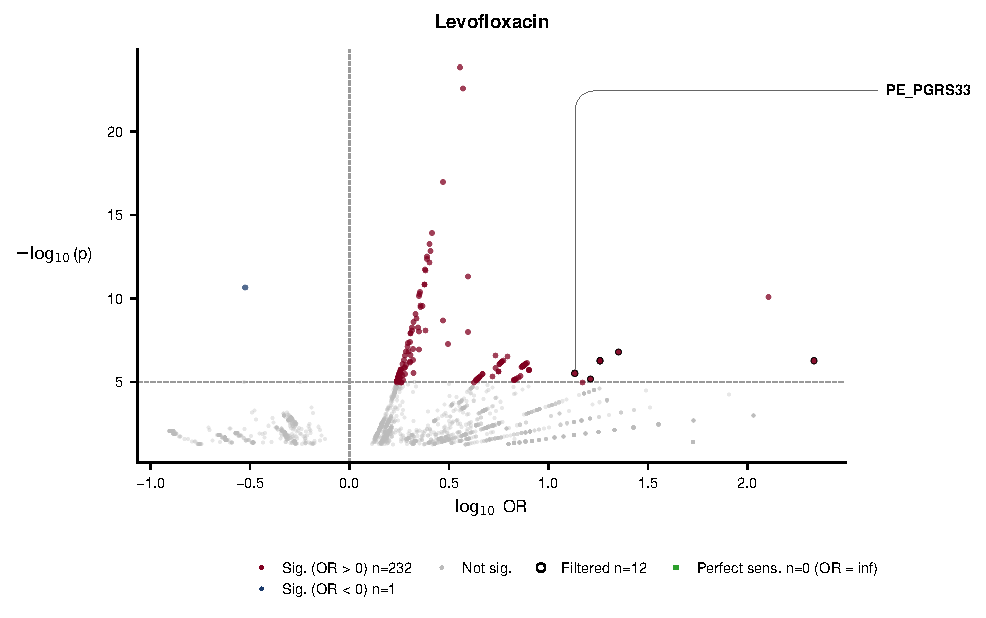
\includegraphics[width=0.45\textwidth]{./figures/plots/levofloxacin_volcano.pdf}
    \hfill
    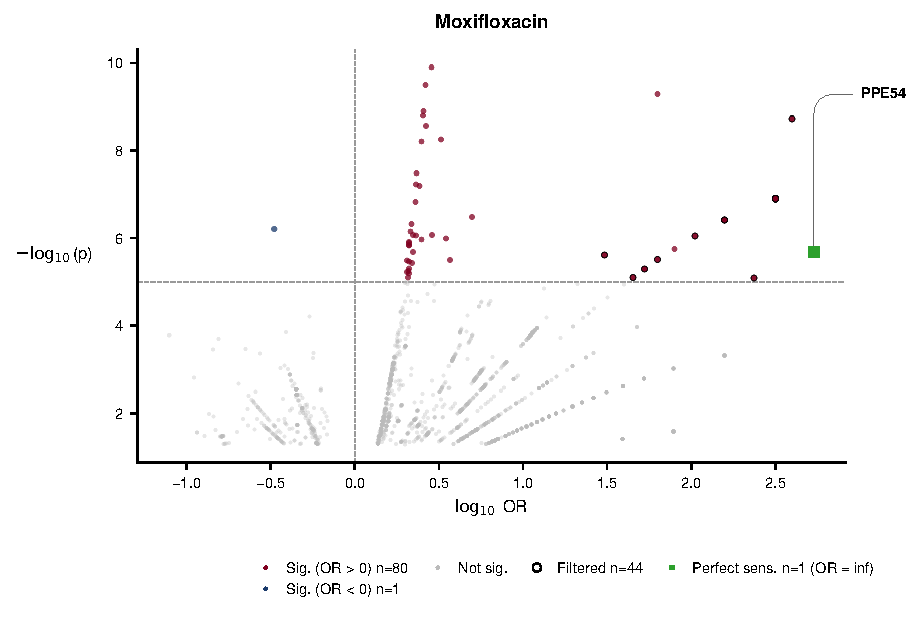
\includegraphics[width=0.45\textwidth]{./figures/plots/moxifloxacin_volcano.pdf}
    \hfill
    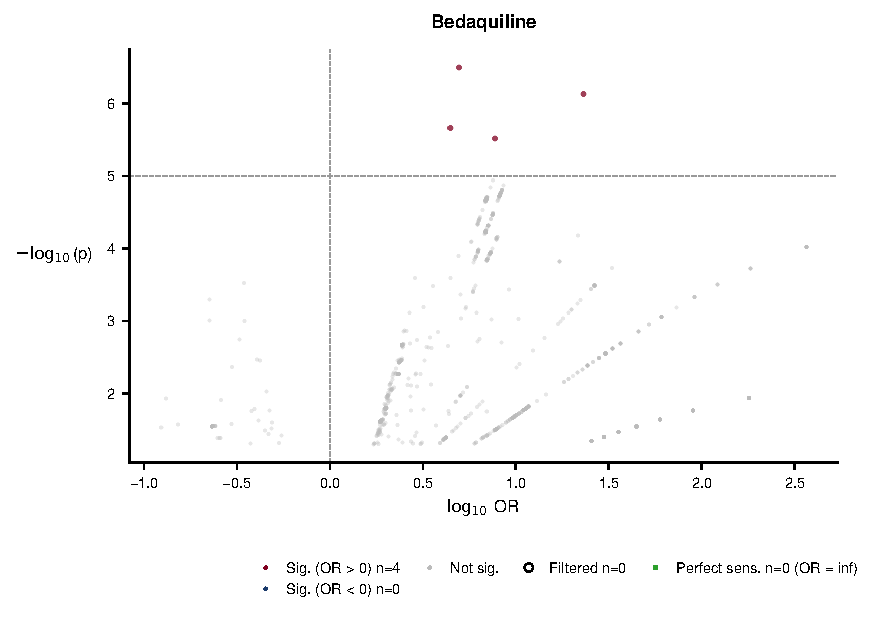
\includegraphics[width=0.45\textwidth]{./figures/plots/bedaquiline_volcano.pdf}
    \hfill
    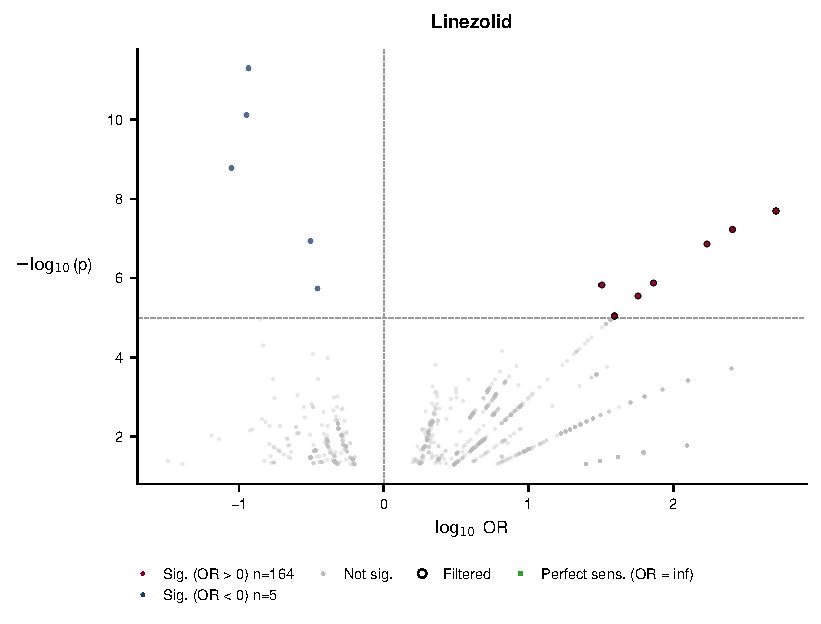
\includegraphics[width=0.45\textwidth]{./figures/plots/linezolid_volcano.pdf}
    \hfill
\end{figure}

\subsubsection{Group B}

Clofazimine unknown mutation is in Rv3254, a conserved hypothetical protein \cite{minato2019genomewide}.

\begin{figure}[H]
    \centering
    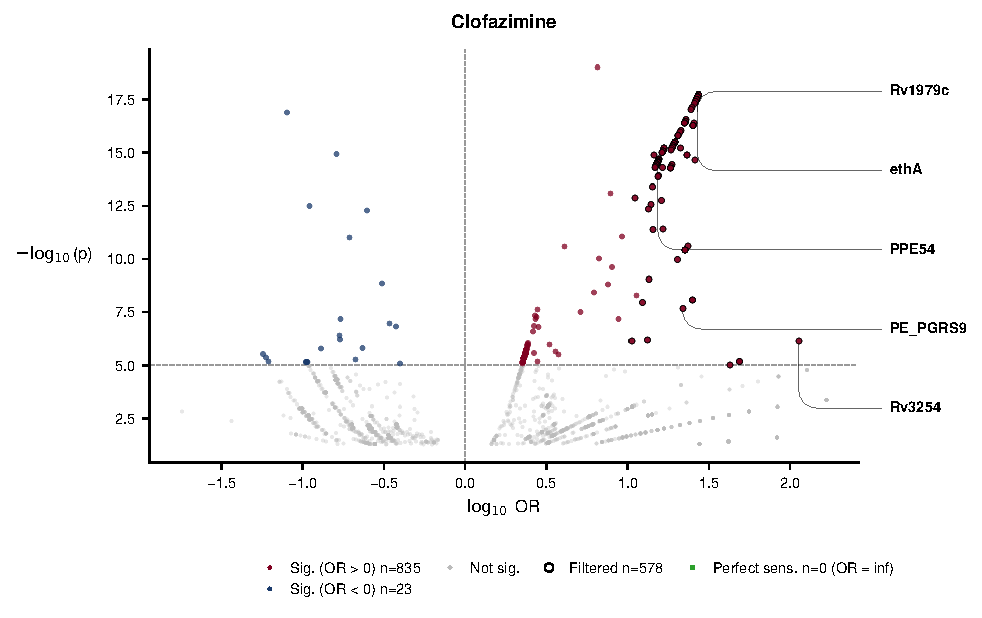
\includegraphics[width=0.45\textwidth]{./figures/plots/clofazimine_volcano.pdf}
    \hfill
    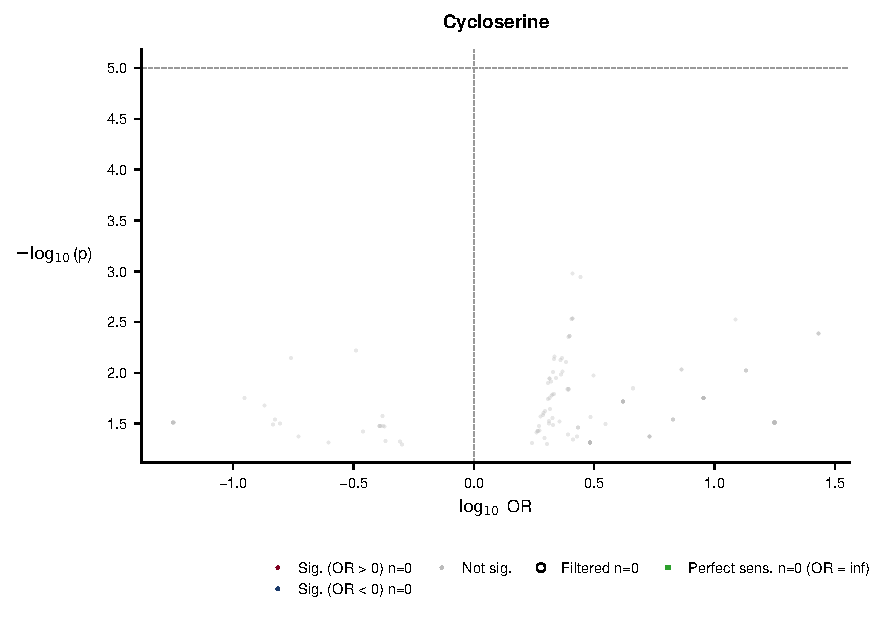
\includegraphics[width=0.45\textwidth]{./figures/plots/cycloserine_volcano.pdf}
    \hfill
\end{figure}

\subsubsection{Group C}

The gene-not-found for ethionamide is the same for isoniazid, 14bp upstream of $fabG1$, which makes sense biologically, since there's cross-resistance \cite{valafar2021systematic}. 

\begin{figure}[H]
    \centering
    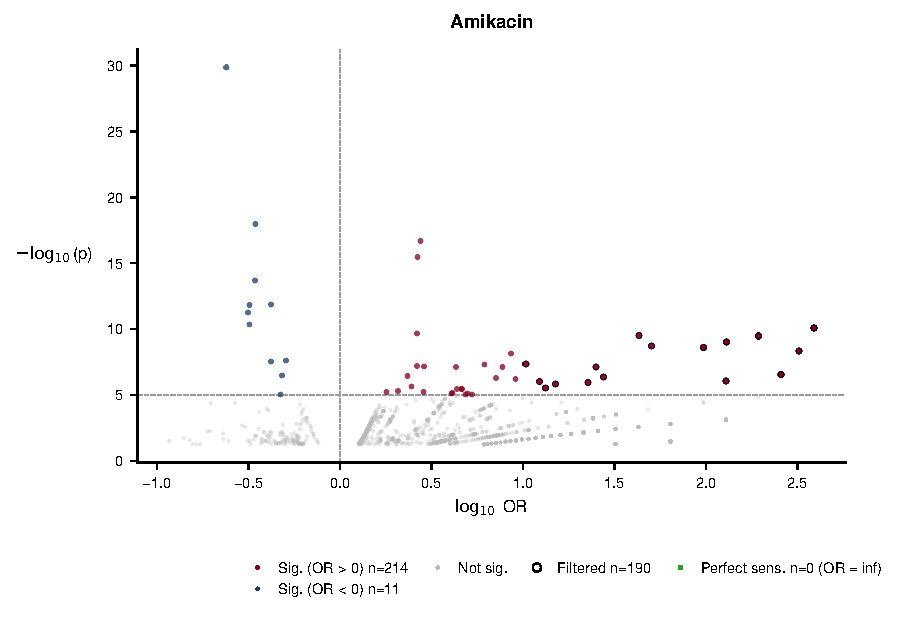
\includegraphics[width=0.45\textwidth]{./figures/plots/amikacin_volcano.pdf}
    \hfill
    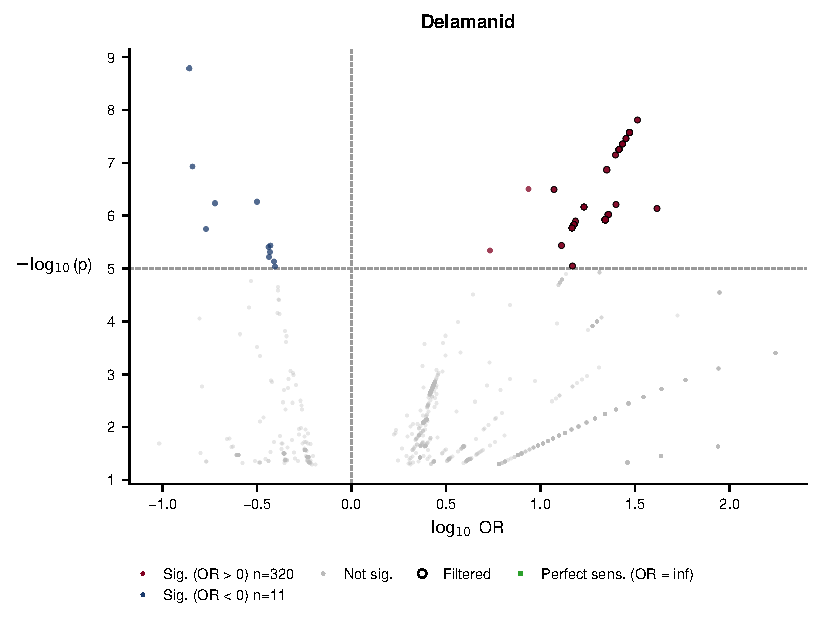
\includegraphics[width=0.45\textwidth]{./figures/plots/delamanid_volcano.pdf}
    \hfill
    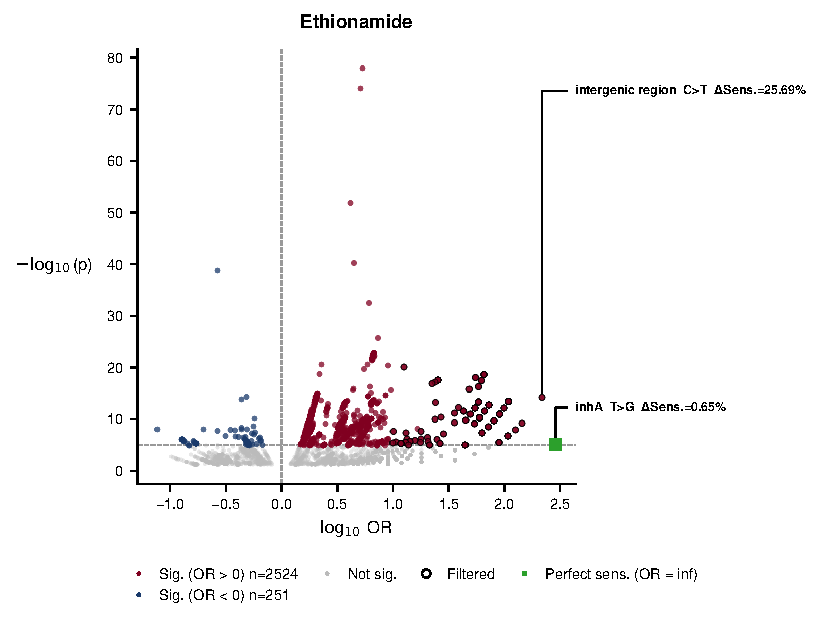
\includegraphics[width=0.45\textwidth]{./figures/plots/ethionamide_volcano.pdf}
    \hfill
    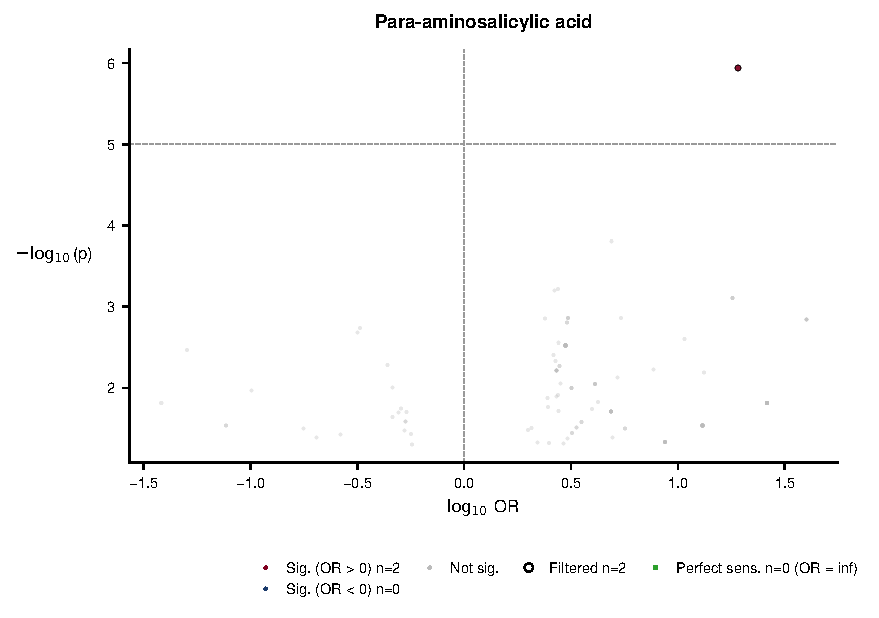
\includegraphics[width=0.45\textwidth]{./figures/plots/para-aminosalicylic_acid_volcano.pdf}
    \hfill
\end{figure}

\subsection{Other drugs}


\begin{figure}[H]
    \centering
    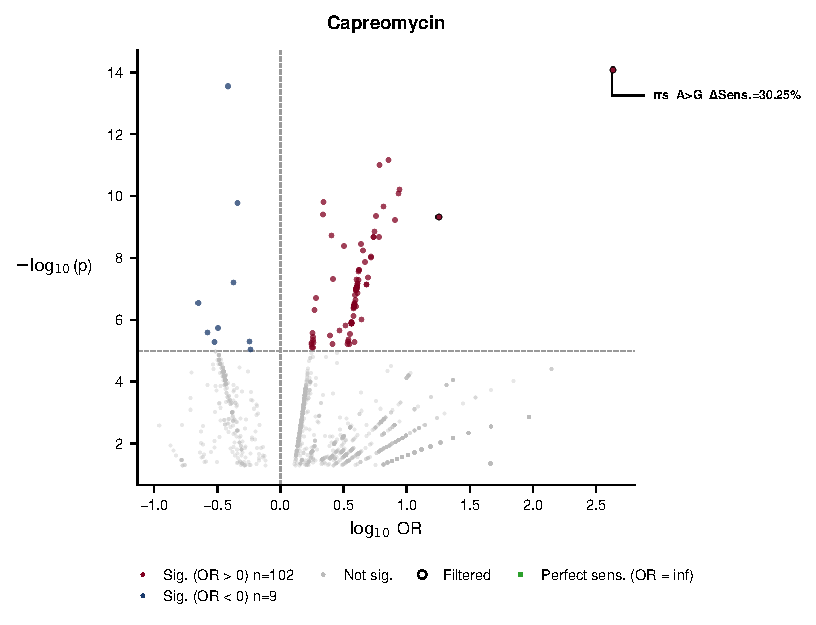
\includegraphics[width=0.45\textwidth]{./figures/plots/capreomycin_volcano.pdf}
    \hfill
    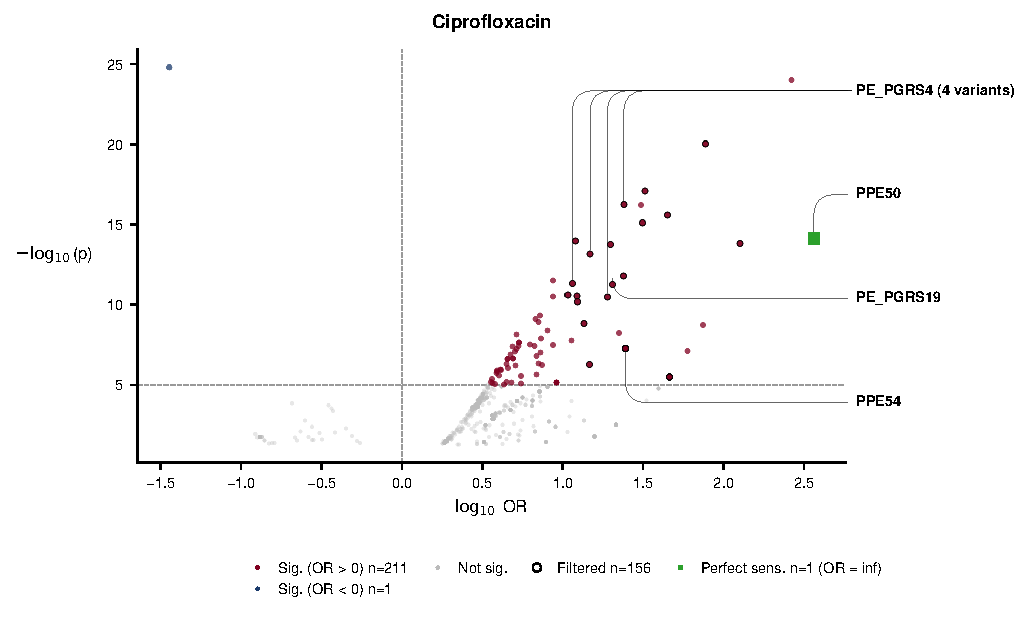
\includegraphics[width=0.45\textwidth]{./figures/plots/ciprofloxacin_volcano.pdf}
    \hfill
    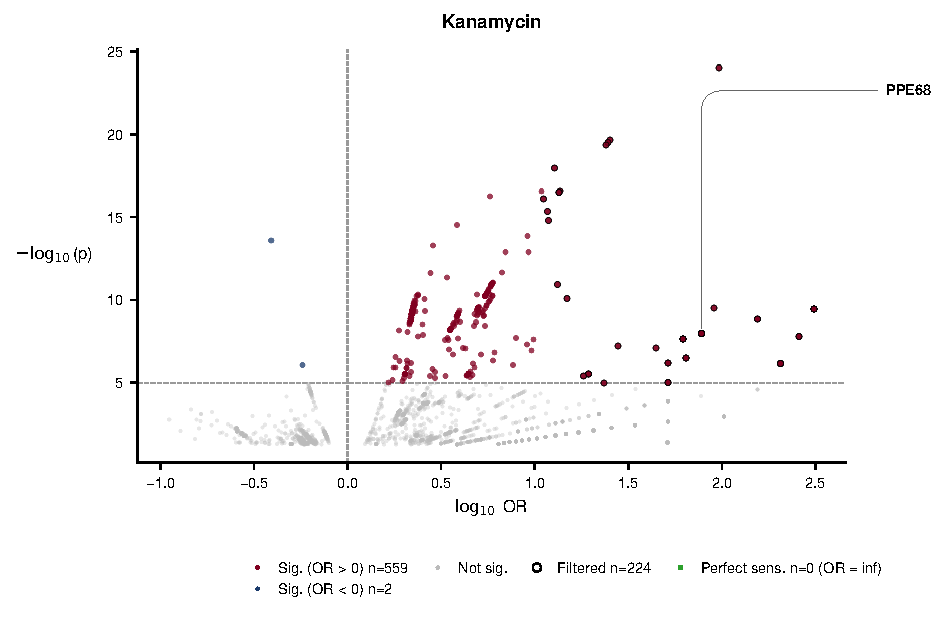
\includegraphics[width=0.45\textwidth]{./figures/plots/kanamycin_volcano.pdf}
    \hfill
    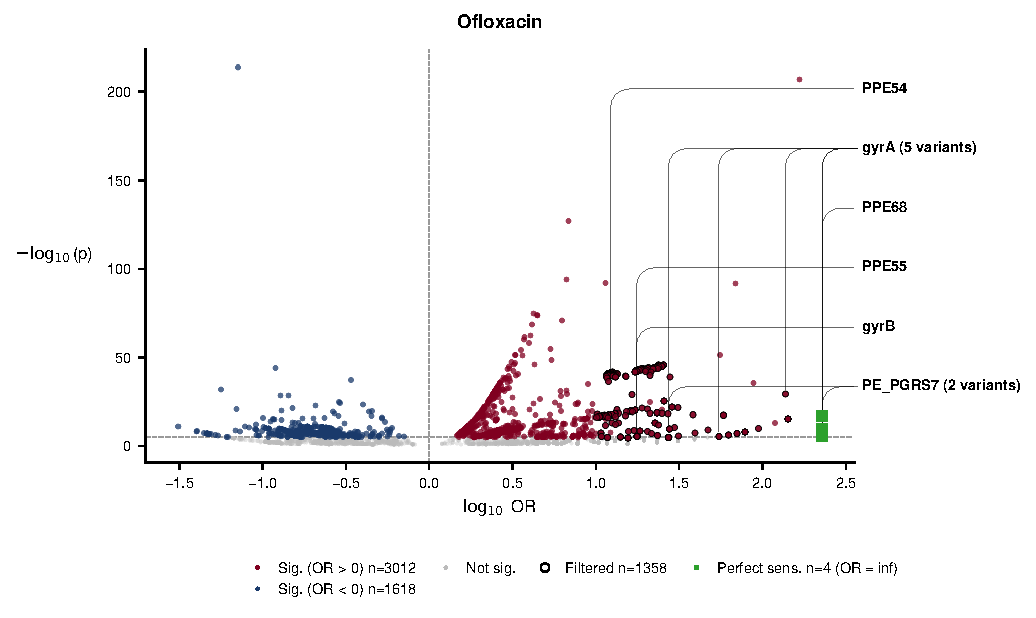
\includegraphics[width=0.45\textwidth]{./figures/plots/ofloxacin_volcano.pdf}
    \hfill
\end{figure}

\input{Chapters/Results/tb_tab.tex}
